% !TeX root =  main.tex

\chapter{Exponential and Logarithmic Functions}

\section{Exponential Functions}
\begin{definition}[Exponential Functions]
For any real number $x$, an exponential function $f$ is a function defined by an equation
$$f(x)=b^x,$$
where $b$ is a positive real number and $b\ne 1$.
\end{definition}
\begin{multicols}{2}
  Let $f(x)=b^x$ be an exponential function. Then
  \begin{itemize}
    \item the domain of $f$ is $(-\infty, \infty)$,
    \item the range of $f$ is $(0, \infty)$,
    \item the $y$-intercept is $(0, 1)$,
    \item $f$ has a horizontal asymptote $y=0$,
    \item $f$ is increasing if $b>1$, 
    \item $f$ is decreasing if $0<b<1$.
  \end{itemize}
  

  Note if $f(x)=ab^x$, then $y$-intercept is $(0,a)$ and $a=f(0)$ is known as the initial value.

  \vfill\null
  \columnbreak

  \begin{tikzpicture}
  \begin{axis}[
  xmin=-3,
  xmax=3,
  ymin=-2,
  ymax=4,
  xtick={-4,-3,...,4},
  ytick={-2,-1,...,5},
  grid=none]
    \addplot[line width=1.5pt,blue, smooth, samples=100, restrict y to domain=-2:6] {3^((x))};
    \addplot[line width=1.5pt,red, smooth, samples=100, restrict y to domain=-2:6] {(1/2)^((x))};  
    \begin{pgfonlayer}{ft}
      \node[align=left] at (-1.2,2) [left] {$y=b^x$,\\ $0<b<1$};
      \node[align=left] at (1.2,2) [right] {$y=b^x$,\\ $b>1$};
    \end{pgfonlayer}
  \end{axis}
  \end{tikzpicture}
\end{multicols}

\begin{example}
  The population of India was about 1.25 billion in the year 2013, with an annual growth rate of about  1.2\%. This situation is represented by the growth function  $P(t)=1.25(1.012)^t$, where $t$ is the number of years since 2013. To the nearest thousandth, what will the population of India be in 2031?
\end{example}

\begin{example}
  In 2006, $80$ deer were introduced into a wildlife refuge. By 2012, the population had grown to $180$ deer. The population was growing exponentially. Write an algebraic function $N(t)$ representing the population $N$ of deer over time $t$.
\end{example}

\newpage

\begin{example}
  Sketch the graph of the function $f(x)=2\cdot 3^{x+1}+1$ by transforming the graph of the function $f(x)=2\cdot 3^x$.
\end{example}

\begin{example}
  Find an exponential function $f(x)=ab^x$ that passes through the points $(-2,6)$ and $(2,1)$.
\end{example}

\begin{example}
  Find an exponential function $f(x)=ab^x$ graphed in the following figure.\\
  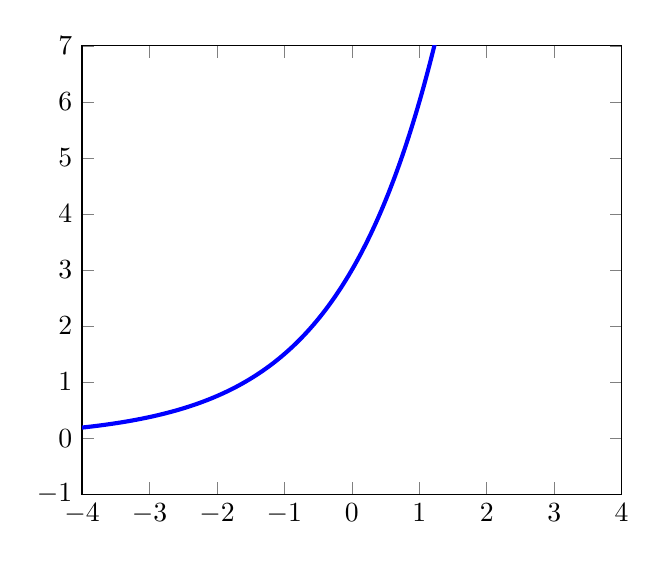
\begin{tikzpicture}
    \begin{axis}[
      xmin=-4,
      xmax=4,
      ymin=-1,
      ymax=7,
      xtick={-6,-5,...,6},
      ytick={-6,-5,...,7}
    ]
    \addplot[line width=1.5pt, blue, smooth, samples=100, restrict y to domain=-2:8] {3*2^(x)};
    \end{axis}
  \end{tikzpicture}
\end{example}

\vspace*{-0.3\textheight}

\newpage

\begin{definition}[The Natural Number $e$]
The natrual number, denoted by $e$, the number that 
${\left (1+\dfrac{1}{n} \right )}^n$ approaches to as $n$ increases without bound. Approximately, $e\approx 2.718282$.
\end{definition}



\begin{example}
  Calculate $e^{3.14}$. Round to five decimal places.
\end{example}

\vspace*{-0.3\textheight}

\begin{note}[Compound Interest]
Let $P$ be the initial amount of the account, known as the principal, $r$ the annual interest rate, and $t$ is the number of years. The balance $A$ after $t$ years is

\begin{itemize}
  \item $A(t)=P{\left (1+\dfrac{r}{n} \right )}^{nt}$ if the interest is compounded $n$ times per year.
  \item $A(t)=Pe^{rt}$ if the interest is compounded continuously ($n\to \infty$).
\end{itemize}
\end{note}
\begin{example}
  We invest $\$3,000$ in an investment account paying $3\%$ interest compounded quarterly, how much will the account be worth in $10$ years?
\end{example}



\begin{example}
  A person invested $\$1,000$ in an account earning $10\%$ per year compounded continuously. How much was in the account at the end of two and a half year?
\end{example}

\newpage

\begin{example}
  A 529 Plan is a college-savings plan that allows relatives to invest money to pay for a child's future college tuition; the account grows tax-free. Lily wants to set up a 529 account for her new granddaughter and wants the account to grow to $\$40,000$ over $18$ years. She believes the account will earn $6\%$ compounded semi-annually (twice a year). To the nearest dollar, how much will Lily need to invest in the account now?
\end{example}

\begin{example}
  $Radon-222$ decays at a continuous rate of $17.3\%$ per day. How much will $100 mg$ of $Radon-222$ decay to in $3$ days?
\end{example}

\newpage
\section*{Exercises}

\begin{exercise}
  A vehicle depriciates according to the formula: $v=27500\left(3.42\right)^{-.04x}$ where $x$ is the age of the car in years. Find the value of the car when it is 14-years old.
\end{exercise}

\begin{exercise}
  Sketch the graph of the function $f(x)=-2\cdot 3^{x-2}+2$.
\end{exercise}

\begin{exercise}
  Find an exponential function $f(x)=ab^x$ that passes through the points $(-2,-6)$ and $(2,-1)$.
\end{exercise}

\newpage

\begin{exercise}
  Find an exponential function $f(x)=ab^x$ graphed in the following figure.\\
  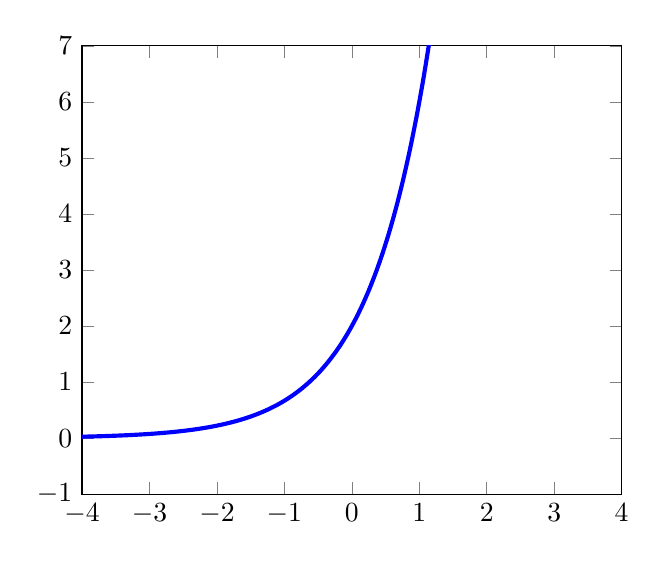
\begin{tikzpicture}
    \begin{axis}[
      xmin=-4,
      xmax=4,
      ymin=-1,
      ymax=7,
      xtick={-6,-5,...,6},
      ytick={-6,-5,...,7}
    ]
    \addplot[line width=1.5pt, blue, smooth, samples=100, restrict y to domain=-2:8] {2*3^(x)};
    \end{axis}
  \end{tikzpicture}
\end{exercise}
\vspace*{-0.25\textheight}

\begin{exercise}
  A wolf population is growing exponentially. In 2011, $129$ wolves were counted. By 2013, the population had reached $236$ wolves. What two points can be used to derive an exponential equation modeling this situation? Write the equation representing the population $N$ of wolves over time $t$.
\end{exercise}

\begin{exercise}
  A scientist begins with $100$ milligrams of a radioactive substance that decays exponentially. After $35$ hours, $50$ mg of the substance remains. How many milligrams will remain after $54$ hours?
\end{exercise}

\newpage

\begin{exercise}
  Consider the function $f(x)=-\dfrac{1}{2e^{-x}+1}$. Find $f(0)$, $f(\sqrt{2})$ and $f(-1)$.
\end{exercise}

\begin{exercise}
  An account is opened with an initial deposit of $\$6,500$ and earns $3.6\%$ interest.
  
  \begin{enumerate}
    \item What will the account be worth in $20$ years if the interest is compounded monthly. 
    \item What will the account be worth in $20$ years if the interest is compounded continuously. 
  \end{enumerate}
\end{exercise}


\newpage
\section{Logarithmic Functions}

\newpage
\section{Properties of Logarithms}

\newpage
\section{Exponential and Logarithmic Equations}

\newpage
\section{Exponential and Logarithmic Models}









